\label{chap-mmds}

\section{Introduction}
\label{s:intro}

Distance sampling (\cite{IDS}, \cite{ADS}) is a suite of methods for estimating the size and/or density of biological populations. The most common approach, referred to as conventional distance sampling (CDS), is based on methods developed by \citeb{buckland92}. A commonly used extension to this methodology allows for the probability of detection to vary with covariates as well as just distance from the observer (multiple covariate distance sampling, MCDS, \cite[chapter 3]{ADS}). 

As was shown in chapter \ref{intro-DS}, estimating the detection function is key to distance sampling. Standard distance sampling methods use the ``key function plus adjustment series'' formulation for the detection function. This can lead to unrealistic functions being fit to data, in particular non-monotone detection functions (as seen in \secref{intro-ds-mono}), in particular in figure \ref{fig1}.

In this chapter, a new class of distance sampling detection function models based on mixtures of simple parametric key functions is introduced. In the next section the models are described and following from that \secref{s:optimization} gives details of the optimization procedure and tricks used. Sections \ref{mmds-sims} and \ref{s:data} show the results of a simulation study and then analysis of real data, respectively. The final section gives some concluding remarks.

\section{Finite mixture model detection functions}

Following on from the definitions of the detection functions given in chapter \ref{intro-DS}, this section shows how from the definition of a mixture model detection function, the likelihood can be found for covariate and non-covariate models of both line and point transect data.

\subsection{Formulation}
\label{s:detfcts}

Denoting the detection function $g$, as before, consider a sum of $J$ mixture (detection function) components $g_j$, scaled by some mixture proportions $\phi_j$:
\begin{equation}
g(x,\mathbf{Z}; \bm{\theta}, \bm{\phi}) = \sum_{j=1}^J \phi_j g_j(x,\mathbf{z}_i; \bm{\theta}_j),
\label{mix-detfct}
\end{equation}
where $\sum_{j=1}^J \phi_j = 1$, $\bm{\phi}$ is a vector of all of the $\phi_j$s. As in chapter \ref{intro-DS}, the distance is denoted $x$, the $\bm{\theta}_j$s are vectors of parameters for function $g_j$, $\bm{\theta}$ is a vector of all of the $\bm{\theta}_j$s and $\mathbf{Z}$ is an $n\times K$ matrix of covariates with rows $\mathbf{z}_i$.

Here all of the $g_j$s are chosen to be half-normal functions, although other monotonic functions such as hazard-rate could be chosen (and the $g_j$s need not all have the same form). A non-covariate $J$-point mixture model would then be written as:
\begin{equation*}
g(x; \bm{\theta}, \bm{\phi}) = \sum_{j=1}^J \phi_j \exp \Big( - \frac{x^2}{2\sigma_j^2} \Big).
\end{equation*}
So here $\bm{\theta} = (\sigma_1, \ldots, \sigma_J)$ and there are no covariates so $\mathbf{Z}$ and $\mathbf{z}_i$ are removed.

\subsubsection{Covariates}

Covariates can be included in a similar way to MCDS (\secref{intro-ds-covar}, \cite[Chapter 3]{ADS}), where the covariates effect the scale parameter ($\sigma$). Here it is assumed that each mixture component has a different scale but that the covariates affect the scale parameters in the same way, in particular this means that the ``intercept'' term in the covariate model is different for each mixture component but the other covariates are estimated jointly for all components. Other more complex models with different covariates in each mixture component may be possible, but only the simplest model is considered here.

Analogously to \secref{intro-ds-covar}, using $i$ to subscript each observation, the formulation for the scale parameter $\sigma_{ij}$, is therefore:
\begin{equation*}
\sigma_{ij} = \exp( \beta_{0j} + \sum_{k=1}^K \beta_k z_{ik}),
\end{equation*}
where $z_{ik}$ is the $k^\text{th}$ covariate for the $i^\text{th}$ observation. As an example, for a 2-point mixture with 1 covariate, the scale parameters take the form
\begin{equation*}
\sigma_{ij} = \exp( \beta_{0j} + \beta_1 z_{i1}),
\end{equation*}
and then $\bm{\theta}_j = (\beta_{0j}, \beta_1)$. If the model was a 2-point mixture, $\bm{\theta} = (\beta_{01}, \beta_{02}, \beta_1)$. Note the similarity to (\ref{intro-ds-covar-model}).

\subsection{Likelihood}

\subsubsection{Line transects}

For line transects, given a set of perpendicular distances $\{x_i; i=1,\ldots,n\}$ and associated covariate vectors $\bm{z}_i$ (the rows of $\mathbf{Z}$), the likelihood is given by:
\begin{align}
\mathcal{L}(\bm{\theta},\bm{\phi}; \mathbf{x},\mathbf{Z}) &= \prod_{i=1}^n f(x_i,\bm{z}_i; \bm{\theta},\bm{\phi}) \notag \\
&= \prod_{i=1}^n \frac{g(x_i,\bm{z}_i; \bm{\theta},\bm{\phi})}{\mu_i} \notag \\
&= \prod_{i=1}^n \frac{\sum_{j=1}^J \phi_j g_j(x_i,\bm{z}_i; \bm{\theta}_j)}{\mu_i} \label{lt-lik}
\end{align}
where $\mu_i$, the effective strip width for an observation with the same covariates as observation $i$, is given by substituting (\ref{mix-detfct}) into (\ref{intro-ds-mu-covar}):
\begin{align*}
\mu_{i} &= \int_0^w  g(x,\bm{Z}; \bm{\theta}) \text{d}x,\\
& =  \int_0^w  \sum_{j=1}^J \phi_j g_j(x,\bm{z}_i; \bm{\theta}_j) \text{d}x,\\
& = \sum_{j=1}^J \phi_j \int_0^w  g_j(x,\bm{z}_i; \bm{\theta}_j) \text{d}x.
\end{align*}

\subsubsection{Point transects}

For point transects, with radial distances $\{r_i; i=1,\ldots,n\}$ and associated covariate vectors $\bm{z}_i$ (the rows of $\mathbf{Z}$), the likelihood is:
\begin{align}
\mathcal{L}(\bm{\theta},\bm{\phi}; \mathbf{r},\mathbf{Z}) &= \prod_{i=1}^n f(r_i,\bm{z}_i; \bm{\theta},\bm{\phi}) \notag \\
&= \prod_{i=1}^n \frac{2 \pi r_i g(r_i,\bm{z}_i; \bm{\theta},\bm{\phi})}{\nu_i} \notag \\
&= \prod_{i=1}^n \frac{2 \pi r_i \sum_{j=1}^J \phi_j g_j(x_i,\bm{z}_i; \bm{\theta}_j)}{\nu_i} \label{pt-lik}
\end{align}
where the effective area of detection for an observation with covariate vector $\mathbf{z}_i$, $\nu_i$ is defined as:
\begin{align*}
\nu_i &= 2\pi \int_0^w  r g(r,\bm{Z}; \bm{\theta}) \text{d}r,\\
& = 2\pi  \int_0^w  \sum_{j=1}^J \phi_j r g_j(r,\bm{z}_i; \bm{\theta}_j) \text{d}r,\\
& = 2\pi \sum_{j=1}^J \phi_j \int_0^w  r g_j(r,\bm{z}_i; \bm{\theta}_j) \text{d}r.
\end{align*}

Parameters are estimated using maximum likelihood. In practise maximization is performed on the $\log$-likelihood (see \secref{s:optimization}) with analytic gradients (appendix \ref{app-mixderivs}).



\subsection{Estimating population size}

As in \secref{intro-ds-pop-size}, estimates of population size can be found from a Horvitz-Thompson-like estimator, all that is needed is the $p_i$s, then (\ref{HT-ds-est}) can be used. For line transects the $p_i$s are given by:
\begin{equation*}
p_i = \frac{1}{w} \sum_{j=1}^J \phi_j \int_0^w  g_j(x,\mathbf{Z}; \bm{\theta}_j) \text{d}x,
\end{equation*}
and for point transects:
\begin{equation*}
p_i = \frac{2\pi}{w^2} \sum_{j=1}^J \phi_j \int_0^w  r g_j(r,\mathbf{Z}; \bm{\theta}_j) \text{d}r.
\end{equation*}
Again, average detection probability for an animal within the covered region, $P_a$ can be used as a standard summary statistic.

%[[[Variances in both $N$ and $P_a$ were found for both non-covariate models (\cite[Appendix C]{yellowbook} TKTKTK) and covariate models (\cite[pp. 38-43]{ADS}) using standard methods set out in the literature. TKTKTK DO SOMETHING ABOUT THIS!!!]]]

\section{Optimization}
\label{s:optimization}

As noted in the literature (for example, \cite[463-480]{BDA}, \cite{robert}), mixture model likelihoods are notorious for being multimodal. This multimodality can cause serious problems when finding MLEs of the parameters. To combat this a mix of optimization routines was to attempt to explore the parameter space as  much as possible.

First, simulated annealing (\cite[pp. 549-554]{numrec}) was used to explore the parameter space (for 500 iterations) then after that a quasi-Newton method (BFGS, \cite{bfgs}) was used to find the maxima (the implementations in the \textsf{R} function \texttt{optim()} were used). These two steps were run 5 times and the model with the lowest AIC was selected as the final model. This two step approach appears to be satisfactory in most cases. To aid the optimization, analytic derivatives were also found; these can be found in appendix \ref{app-mixderivs}.

\subsection{Parametrization of the mixture proportions}

When using 2-point mixtures, the constraint that the mixture proportions must sum to unity is enforced by definition (since $\phi_2=1-\phi_1$). However, in $J$-point mixtures when $J>2$ ensuring that the proportions sum to 1 is not guaranteed. The obvious way to get around this would be to add a penalty to the likelihood, should the optimization procedure propose values for the $\phi_j$s that are not in accordance with this condition. This approach is not appealing since the point of using mixtures here is to avoid penalizing or constraining the likelihood if possible. Given the problems inherent in optimizing mixture likelihoods in general, adding penalization only further complicates matters. Instead, a parametrization (due to David Borchers) is used for the mixture proportions which yields $\phi_j$s that comply.

Rather than estimating the $\phi_j$s, estimate $\alpha_p$s, where the relationship between the two is:
\begin{equation*}
\phi_j = F(\sum_{p=1}^j e^{\alpha_p}) - F(\sum_{p=1}^{j-1} e^{\alpha_p}) \qquad \text{for } 1\leq j \leq J-1
\end{equation*}
and
\begin{equation*}
\phi_J = 1-\sum_{j=1}^{J-1} \phi_j
\end{equation*}
where $F$ is any continuous CDF on $(0,\infty]$. Exponentiation ensures that $e^{\alpha_p}\geq0$, so $\alpha_p$ may lie anywhere on the real line, allowing unconstrained optimisation. Summing these orders the $\phi_j$s, since only offsets are estimated. Finally, using the cumulative density function ensures that the $\phi_j$s sum to $1$. In practise the $\text{Gamma}(3,2)$ CDF is (somewhat arbitrarily) used. Figure \ref{mmds-phifig} illustrates the relationship.

\begin{figure}
\centering
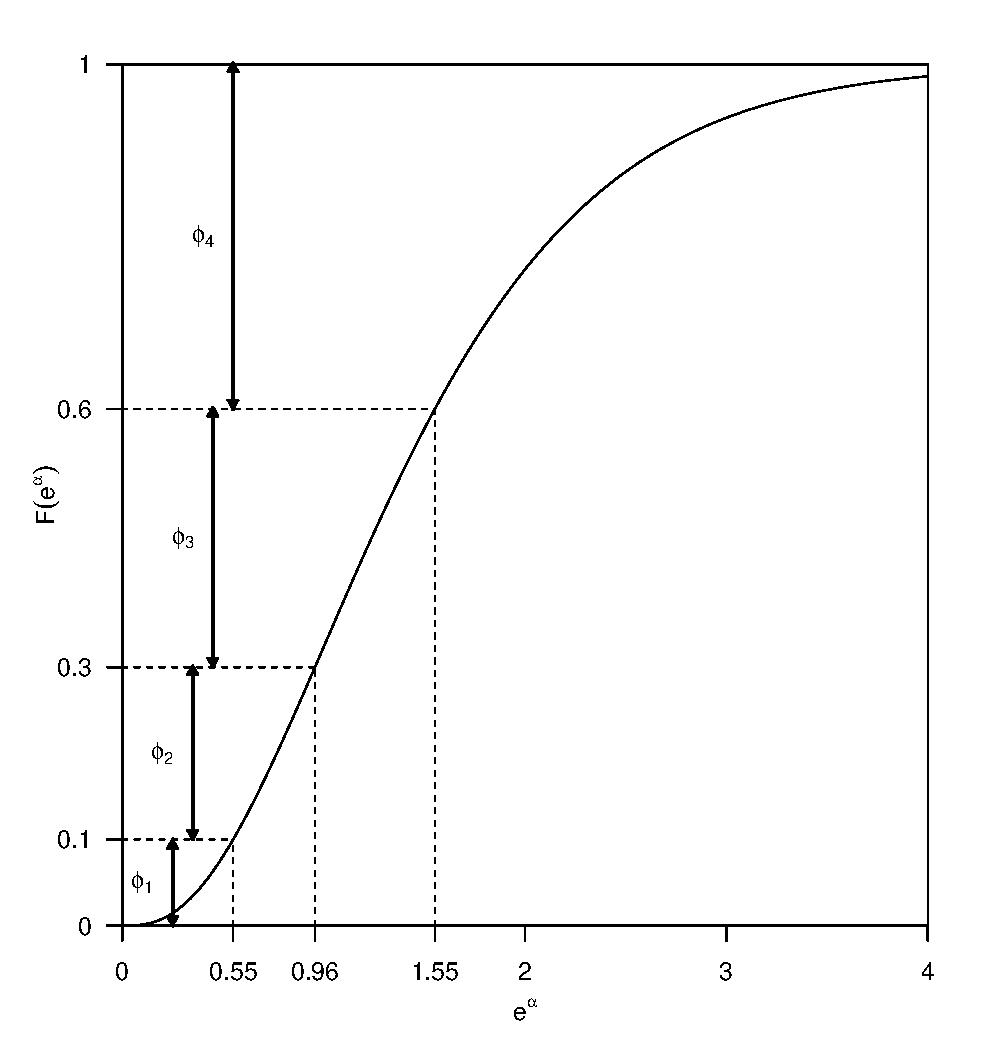
\includegraphics[width=3.5in]{mix/figs/phidia.pdf}
\caption{Illustration of the relationship between the mixture proportions, $\phi_j$ and the quantites estimated in the optimization procedure $\alpha_p$.}
\label{mmds-phifig}
\end{figure}

To transform from the $\phi_j$s back to the $\alpha_p$s by simply re-arranging the above expression.
\begin{equation*}
\alpha_p = \log_e \Big(F^{-1}\Big(\phi_j + F(\sum_{p=1}^{j-1} e^{\alpha_p})\Big) - \sum_{p=1}^{j-1} e^{\alpha_p}\Big).
\end{equation*}
Note that only as many $\alpha_p$s are needed as $\phi_j$s, so no additional parameters are required.

\subsection{Starting values}

\citeb{beavers98} give a method for estimating starting values for the scale parameter of a half-normal detection function. In the non-covariate case, the estimate is given as the intercept parameter from intercept only regression on $\log(x+\frac{w}{1000})$ (where $w$ denotes the truncation distance, as above). For covariate models, the equation used for the $\sigma$ is used in the regression and the estimated parameters from the linear regression are used as the starting values for the $\beta$s.

A similar approach can be use in the mixture case by dividing the sorted distances into $J$ equal parts. For each of these parts a Beavers and Ramsay-type estimate is used for the $\beta$s. The $\phi_j$ had starting values of $1/J$ since there is no reason \textit{a priori} to believe anything else.

\section{Simulations}
\label{mmds-sims}

Extensive simulations were carried out to ensure that both parameters could be recovered and that abundance estimates were unbiased. The latter is more important than the former since our primary interest is estimating abundance. Since (as has been illustrated in \secref{intro-ds-pop-size}) the abundance depends only on the probability of detection, this was used as a target quantity to estimate and compare the results. Each simulation involved generating 200 replicate datasets from a specified mixture model using rejection sampling, fitting each dataset with 1-, 2-, and 3-point mixture models for the detection function, and in each case recording estimated (average) probability ($p$ for non-covariate situations, $\hat{P}_a$ for covariates) of detection from the model with the lowest AIC.

\subsection{Rejection sampling scheme to simulate distances}

Before going into the details of the simulation a method for generating distance data from mixture detection functions needed to be found. The cumulative distribution function of the mixture model cannot be inverted so rejection sampling (also known as the accept-reject algorithm, \cite[pp. 51-53]{montecarlostats}) was used. This is rather wasteful computationally since the proposal distribution used here is only a uniform on $(0,w)$, a proposal closer to the target could be used to increase the speed (however, this is not a major concern here). Note that direct simulation from half-normals is not possible since it is the detection functions which are mixtures rather than the PDFs. The rejection sampling scheme for $n$ samples from a mixture model detection function is as follows. 

Until there are $n$ samples, perform the steps:
\begin{enumerate}
\item Generate $X \sim \text{Uniform}(0,w)$. 
\item Generate $U \sim \text{Uniform}(0,1)$.
\item Accept $X$ as coming from the PDF of distances, $f$, if 
\begin{equation*}
U \leq \frac{f(X,\mathbf{z}_i; \bm{\theta}, \bm{\phi})}{(1/w) M}\\
\end{equation*}
where $M$ is the maximum of $f$ and $1/w$ is the PDF of the proposal for $X$. Acceptance means that $X$ is within the ``envelope'' of $f$.
\end{enumerate}

In the line transect case, it is known that that the maximum value of $f$ is $1/\mu$ (since $\mu=1/f(0)$ and f(0) is the maximum of $f$), so $M=1/\mu$ (or $1/\mu_i$ in the covariate case). For point transects the maximum value of $f$ is unknown, so for each simulation the maximum was found via numerical optimization (using the \textsf{R} function \texttt{optimize()}). 

\subsection{Simulation settings}

Clearly there are many options in terms of which simulation settings to use. Four sets of simulations were run, which give a fairly broad range of possible scenarios.
\begin{enumerate}
	\item \textit{Non-covariate 2-point detection functions for line transect data}. Four different detection functions were tested, and are shown in the first row of figure \ref{sim-detfcts}. The first two are deliberately fairly easy to fit. The third should be harder, testing the behaviour of the model when one of the parameters is hard to estimate (the scale parameter of one of the mixture components is very large relative to the truncation distance). Finally, the fourth detection function has a large spike, which is similar to that in some of the data analysed in section \ref{s:data}.
	\item \textit{Non-covariate 2-point detection functions for point transect data}.  The detection functions were as above, with data generated as if it came from point transects. The PDFs are given in the second row of figure \ref{sim-detfcts}; the dotted lines indicate the component PDFs scaled such that the area under each curve is one.
	\item \textit{Non-covariate 3-point detection functions for line transect data}. Two different models for the detection functions were used. They are shown in the third row of figure \ref{sim-detfcts}. The first is much like the second line transect detection function, enabling us to investigate the efficacy of model selection. The second is a more complex shape that could only be created using a 3-point mixture; it has the added complication (as with the third line transect simulation) that one of the components may be non-identifiable.
	\item \textit{Covariate 2-point detection functions for line transect data}. Two different models were tested, the first of which has a binary factor covariate: half of the observations had covariate value 1 and half had covariate value 0. The second model had a continuous covariate, whose values were generated from a standard normal distribution function. Detection functions are shown in the fourth row of figure \ref{sim-detfcts}, along with the marginal detection functions for the levels/quantiles of the covariates. One goal was to test the properties of the estimator in the presence of covariates, and for these runs covariates were included in all models.  However, it is also interesting to evaluate the performance of the mixture model formulation in cases where a covariate affects detectability but the covariate is not available to the surveyor. Therefore the same simulated datasets were fit with mixture models that did not include covariates, and compared the resulting estimates to their with-covariate counterparts.
\end{enumerate}

\begin{figure}
\centering
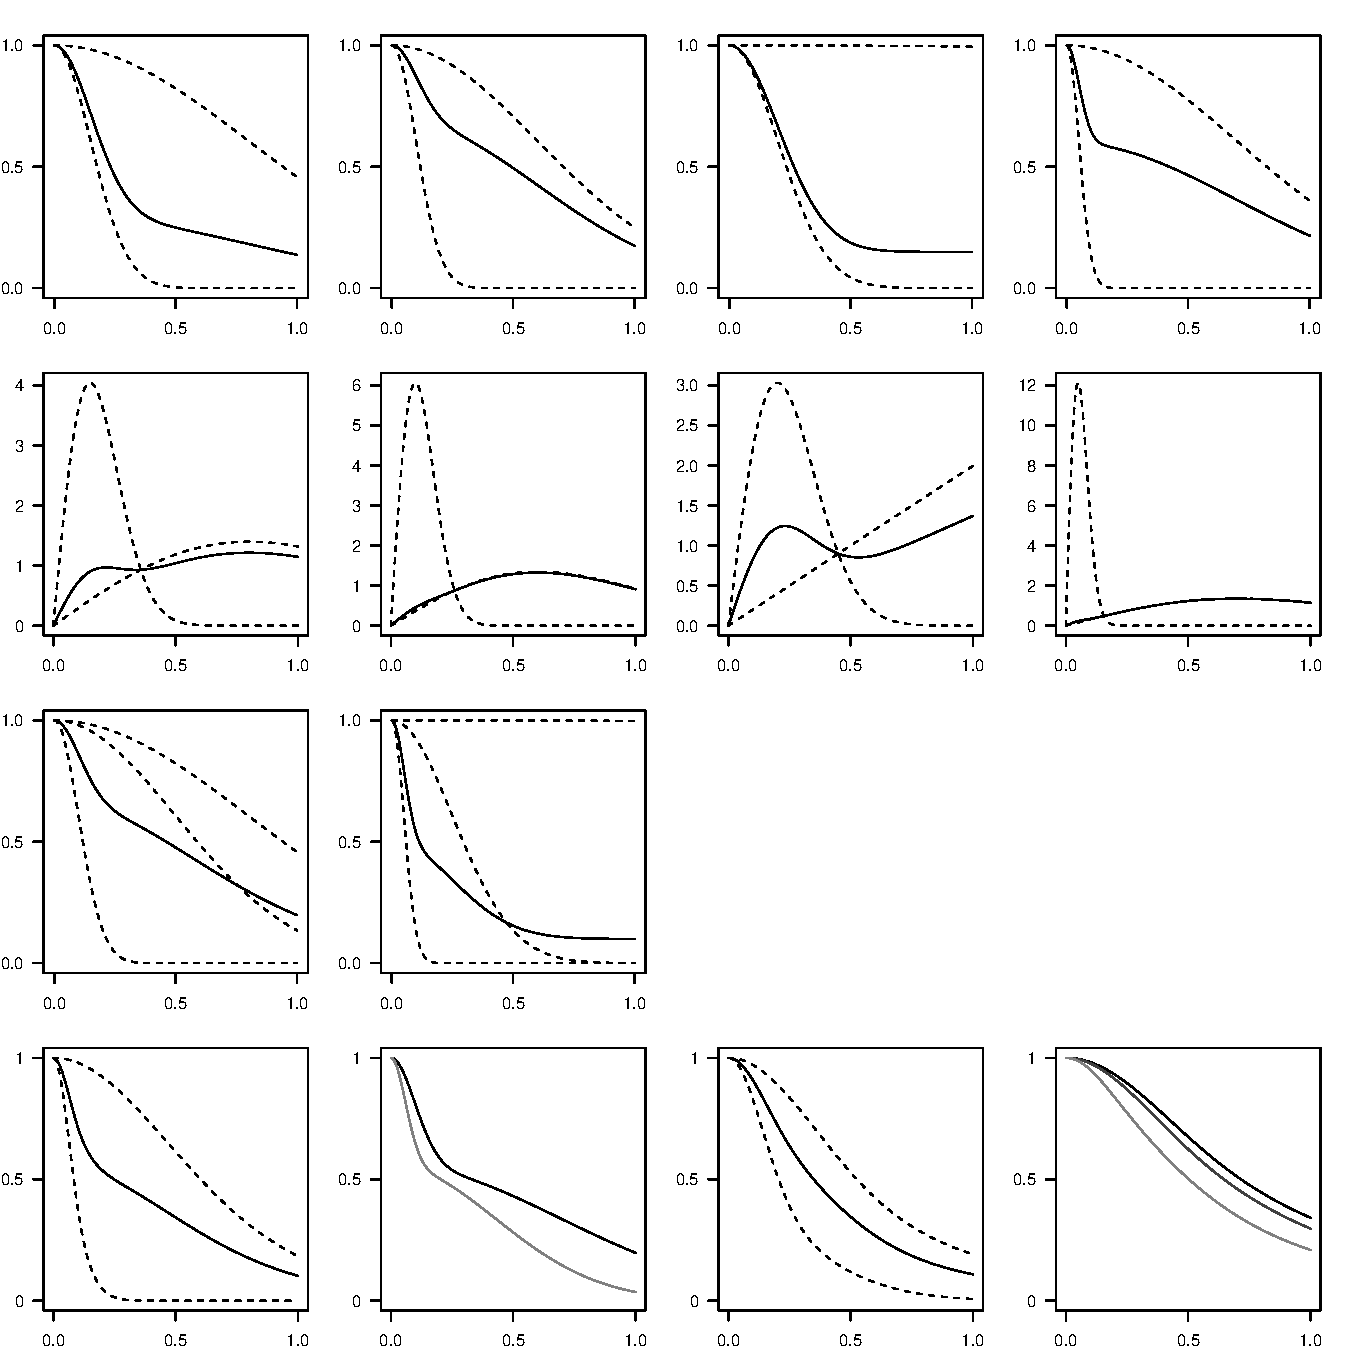
\includegraphics[width=\textwidth]{mix/figs/sim-detfct.pdf}
\caption{Plots of the models used in the simulation. Top row: detection functions for the line transect simulations with no covariates (solid lines) and their constituent mixture components (dashed lines). Second row: PDFs for the point transect simulations with no covariates (bold lines), with associates component PDFs, rescaled so the area under each curve is one; the detection functions are as in the top row. Third row: two 3-point mixtures for non-covariate line transect data, again with components as dashed lines. Fourth row, two covariate models, the first two panels are for a binary covariate, the second two for a continuous covariate; first panels in each pair show the detection function averaged over the covariates (along with the mixture components, similarly averaged) and the second panels show marginal detection functions with the levels (or quantiles) of the detection function.}
\label{sim-detfcts}
\end{figure}

\subsection{Results}

Results from the simulation study are shown in figure \ref{sim-boxplots}, the boxplots therein are of the estimated detection probability ($\hat{p}$) for non-covariate models and average detection probability ($\hat{P}_a$) for covariate models. The number under each boxplot gives the proportion of AIC best models that were of the same form as the true model (i.e. same number of mixture components and the same covariates). For the first row (line transects with no covariates) we can see that in scenarios 1 and 3, both the true model and true probability of detection were found at even low sample sizes, whereas in scenarios 2 and 4 there was a positive bias in the estimates of the probability of detection as well as a lower proportion of ``correct'' models being selected by AIC. In scenario 2 and 4 most of the weight (0.7 and 0.6, respectively) is given to the larger mixture component, thus the smaller component is swamped; this would make the simulated data look as if it were generated from a 1-point mixture.

This effect can also be seen in the point transect simulations, but more severely. In this case one can see from the second row of figure \ref{sim-detfcts} that the PDFs of the distances look very much like only one of the components of the mixture. Fitting only a 1-point mixture to data from a 2-point mixture has lead to a positive bias in the detection probabilities, however this is only to expected given that data generated from such models would look like a 1-point mixture.

The 3-point mixtures show that detection function specified in scenario 1 can be easily represented using a smaller number of mixture terms. At sample sizes of 120 and lower, a 1-point mixture model dominated (around 150 of the AIC selected models were 1-point mixtures) then at the two higher sample sizes, 2-point mixtures dominated. Scenario 2 seemed more like a ``true'' 3-point data set, although only at the two larger sample sizes was a 3-point model selected more than half of the time. Interestingly at the lower sample sizes, a 2-point mixture was selected more often than 1-point (137, 173 and 182 times for the lowest three sample sizes). This effect may be due to the large, potentially non-identifiable, scale parameter being confounded with the other parameters, although this did not appear to be problematic in the scenario 2 of the line transect non-covariate models, above.

The covariate models again show an initial positive bias in $\hat{P}_a$ but do still converge to the true value at higher sample sizes. The numbers beneath the boxplots mask rather more than in the other models, since model selection was performed on not only the number of mixtures but also as to whether covariates were included in the model. Further analysis shows that at the larger two sample sizes we see that the ``true'' model is selected almost all of the time. However,  at smaller sample sizes we see more interesting behaviour. For scenario 1, at the two lowest sample sizes a 1-point non-covariate model dominates, followed by 1-point with covariates, then 2-point covariate and 2-point non-covariate. So, as one would expect, the simplest two models are selected most, but the added information from the covariates means that the 2-point covariate is selected ahead of the 2-point non-covariate. At sample size 120, the 1- and 2-point covariate models are both selected about 70 times, and the non-covariate 1- and 2-point models about 30 times. Contrary to expectations the 3-point mixtures are barely selected at all (with or without covariates) leading to the conclusion that the covariates cannot simply be substituted by further mixture terms, even in the binary covariate case. Scenario 2 shows a slightly different picture; the non-covariate models are selected less, even at lower sample sizes (the 1-point covariate model was selected 90 times a the lowest sample size) which might be expected given that scenario 2 included a continuous covariate. As was the case for scenario 1, the 3-point models were barely selected at all. In both scenarios there seems to be a bite point between a sample size of 120 and 480 where the correct model is selected almost every time.
	

\begin{figure}
\centering
\includegraphics[width=6.5in]{mix/simulations/pa-plot.pdf}
\caption{Simulation results: boxplots of the estimated detection probabilities for the best model (by AIC score). Layout is as in figure \ref{sim-detfcts}. Grey lines indicate the true value of the average detection probability. Numbers underneath each boxplot give the proportion of AIC best models that were of the same form as the model that the data was simulated from (e.g. in covariate case 1 the proportion of AIC best models that were two point mixtures that included the covariate in the model).}
\label{sim-boxplots}
\end{figure}


\section{Real data}
\label{s:data}

Given the performance of the method in simulation, four data sets were analysed using the method. They were chosen because either they exhibited non-monotonicity (\cite{williams}, \cite{pike}), were particularly spiked (\cite{ants}) or were sufficiently big that it was though they might support a mixture with many components (\cite{amakihi}). Between them they cover both covariate and non-covariate data from line and point transect surveys on boats and on foot.

\subsection{Williams and Thomas (2007) cetacean survey}

\citeb{williams} study several species of cetaceans off the coast of British Columbia. Here data for three of the species are re-analysed: harbour seal (in water), harbour porpoise and humpback whale (with truncation at 500m, 500m and 2000m respectively). Results are summarised in table \ref{williams-table} and detection functions for the best (in an AIC sense) models are shown in figure \ref{williams-detfcts}.

\begin{table}
\centering
\begin{tabular}{c c c c c c}
Species & Model & AIC & $\hat{P_a}$ & $\% CV \hat{P_a}$ & K-S $p$\\
\hline
Harbour seal & Hn+$\cos(2)$ (W\&T) & 2771.05 & 0.425 & 7.55 & 0.515\\
(in water) & Hn 2-pt  & 2769.86 & 0.335 & 14.8 & 0.945\\
Harbour porpoise & Hr (W\&T) & 690.66 & 0.212 & 32.0 & 0.99\\
 & Hn 2-pt & 692.09 & 0.254 & 17.5 & 0.99\\
Humpback & Hn+$\cos(2)$ (W\&T) & 1033.06 & 0.386 & 12.64 & 0.672 \\
 & Hn 2-pt & 1035.94 & 0.381 & 15.6 & 0.649 \\
\end{tabular}
\caption{Comparison of the results for the \citeb{williams} data. W\&T indicates the results reported in \citeb{williams}, other results are from mixture models where the number of mixture components was selected by AIC. $\cos(x)$ indicates a Cosine adjustment of order $x$.}
\label{williams-table}
\end{table}

In each case a 2-point mixture was selected by AIC to be the best model. The mixture models for the harbour porpoise and the humpback both did not perform as well as the models selected in \citeb{williams}. However, for the harbour porpoise the AIC is only different by 2, the detectability is very similar and the \%CV is lower, so it does not appear that much is lost by using the mixture model. In the case of the humpback, the fitted detection function is monotone, which was not the case in \citeb{williams}; this added to the fact that there is again not a huge difference in results, leads us to believe that mixture models for the detection function can be useful. Finally, for the harbour seal data, the mixture model had a better AIC than the half-normal with cosine adjustments of order 2 which was selected in the paper. The goodness-of-fit was also significantly better than the result given in \citeb{williams}.

\begin{figure}
\centering
\includegraphics[width=\textwidth]{mix/analyses/williamsplots.pdf}
\caption{Plots of the detection functions fit to the \citeb{williams} data. In each case the best model by AIC was a 2-point mixture. Dashed lines show the mixture components.}
\label{williams-detfcts}
\end{figure}


\subsection{Wood ants in the Abernethy forest}

\citeb{ants} analyse data on two species of wood ant (\textit{Formica aquilonia} and \textit{Formica lugubris}) in the Abernethy Forest in Strathspey Scotland over the period of August--September 2003. The number of nests sighted was 150 out to a distance of 72.04m from the track line, although 45\% of the nest sightings lay within 4m of the line. As part of their analysis several different truncation distances were used and larger truncation distances led to large variance in the encounter rate estimates and hence in overall abundance estimates (\cite{ants}). This is due to the spike caused by the large number of detections close to the line.

As well as distances, three covariates were recorded: habitat type (\texttt{habitat}, a four level factor, the size (calculated as half-width multiplied by height) of each nest (\texttt{nest.size}, continuous variable) and whether \textit{Formica aquilonia} or \textit{Formica lugubris} were observed (\texttt{species}, a two level factor). In order to avoid numerical problems due to large values of the nest size, the variable was standardised.

As can be seen from table \ref{big-results-table}, the best model by AIC was a 2-point mixture with nest size and habitat as covariates. This is not that surprising given the best CDS model (selected by AIC) in Distance was a hazard-rate with the same covariates. What is rather surprising is that the best mixture model had a better AIC than the hazard-rate, even though it has 1 more parameter. This is particularly encouraging since one might expect that mixtures would give good fits but would not achieve lower AIC scores due to the number of parameters required.

\begin{figure}
\centering
\includegraphics[width=\textwidth]{mix/analyses/ants-nesthab.pdf}
\caption{Plot of the detection functions for the AIC best model for the ants data set (2-point mixture with nest size and habitat as covariates). The first panel shows the average detection function (dashed lines are the two mixture components of the detection function, averaged over covariate values). The second and third panels show the quantiles (25\%, 50\% and 75\%) of nest size and the levels of habitat type respectively.}
\label{ants-nesthab}
\end{figure}

\subsection{Long-finned pilot whales}
\label{mix-pilotwhales}

\citeb{pike} analyse data on long-finned pilot whales (\textit{Globicephala melas}). There were 84 pods sighted as part of the NASS-2001 survey (of which the pilot whale was not a target). The Beaufort sea state was recorded as a covariate during the survey and enter the model as either a continuous variable (\texttt{BSS}), 6 level factor (\texttt{BSS}, as a factor), a 2 level factor (\texttt{BSS3}) or a 3 level factor (\texttt{BSS2}).

A model was fit with each of these covariates, as well as a model with no covariates. A summary of the results is given in table \ref{big-results-table} and the detection function for the best model is shown in figure \ref{danpike-detfct}.

\begin{figure}
\centering
\includegraphics[width=0.75\textwidth]{mix/analyses/danpike-bss2.pdf}
\caption{The (AIC) best model for the long-finned pilot whale data -- a 2-point mixture model detection function with Beaufort sea state. Left: the average detection function, right: the marginal detection function with the levels of \texttt{BSS2}.}
\label{danpike-detfct}
\end{figure}

The best model by AIC score was a 2-point mixture with \texttt{BSS2} as a covariate. Figure \ref{danpike-detfct} shows the average detection function and the marginal detection function with the levels of \texttt{BSS2}. The plot looks significantly better than the one shown in figure \ref{fig1}.

\subsection{Amakihi}
\citeb{amakihi} analyse data on the Hawaii Amakihi (\textit{Hemignathus virens}). The data consist of 1485 observations on the bird ($n=1243$ after truncation at 82.5m), collected at 41 point transect from July 1992 to April 1995. Data was also collected on three covariates: the observer (\texttt{obs} , a three level factor), minutes after sunrise (\texttt{mas}, continuous) and hours after sunrise (\texttt{has}, a six level factor).

\begin{figure}
\centering
\includegraphics[width=\textwidth]{mix/analyses/amakihi-om.pdf}\\
\includegraphics[width=0.4\textwidth]{mix/analyses/amakihi-om-pdf.pdf}
\caption{Plots of the (AIC) best model for the amakihi data. Top row: detection function averaged over covariates (dashed lines are each mixture component averaged over covariates), marginal detection function showing the levels of observer (averaged over the values of minutes after sunrise) and marginal detection function for the quantiles minutes after sunrise (averaged over the levels of observer). Bottom row: PDF of distances averaged over the covariate values.}
\label{amakihi}
\end{figure}

Best mixture model according to AIC was a two point mixture with observer and minutes after sunrise as covariates (shown in figure \ref{amakihi}), closely followed by the model with only observer as a covariate (see table \ref{big-results-table}). In this case a hazard-rate with observer and minutes after sunrise as covariates beat the mixtures in AIC terms. This is not too surprising given that the mixtures use one more parameter than a hazard-rate in this situation. It is encouraging that there is such a small difference in AIC, and that covariate mixture models were selected despite the large number of parameters that such models entail.


\begin{table}
\centering
\begin{tabular}{c l c c c}
Model & Covariates & AIC & $\hat{P_a}$ & K-S $p$\\
\hline
 & ($i$) \textit{Ants} & & &  \\
Hn 2-pt & None & 754.61 & 0.183 & 0.96 \\
Hn 2-pt & \texttt{habitat} & 751.27 & 0.150 & 0.97 \\ 
Hn 2-pt & \texttt{species} & 756.59 & 0.184 & 0.94 \\  
Hn 2-pt & \texttt{nest.size} & 741.64 & 0.214 & 0.76 \\   
Hn 2-pt & \texttt{habitat} + \texttt{species} & 749.05 & 0.152 & 0.94\\ 
Hn 2-pt & \texttt{habitat} + \texttt{nest.size} & \textbf{737.27} & 0.179 & 0.72\\
Hn 2-pt & \texttt{nest.size} + \texttt{species} & 741.92 & 0.210 & 0.77\\
Hn 2-pt & \texttt{nest.size} + \texttt{species} + \texttt{habitat} & 739.77 & 0.178 & 0.68 \\
Hr & \texttt{habitat} + \texttt{nest.size} & 745.2 & 0.194 & 0.95\\
 & ($ii$) \textit{Long-finned pilot whales} & & & \\
Hn 2-pt & None & 1298.42 & 0.295 & 0.95 \\
Hn 2-pt & \texttt{BSS} & 1286.6 & 0.209 & 0.82 \\
Hn 2-pt & \texttt{BSS2} & \textbf{1284.99} & 0.211 &  0.95\\
Hn 2-pt & \texttt{BSS3} & 1296.27 & 0.27 & 0.99 \\
Hn 2-pt & \texttt{BSS} (cont.) &  1286.26 & 0.152 & 0.84\\
Hn 1-pt + $\cos(2)$& \texttt{BSS} (cont.) & 1296 & 0.37 & 0.319 \\
 & ($iii$) \textit{Amakihi} & & & \\
Hn 2-pt & None & 10805.48 & 0.283 & 0.12 \\
Hn 2-pt & \texttt{obs} & 10778.69 & 0.289 & 0.04\\
Hn 2-pt & \texttt{has} & 10807.19 &  0.282 & 0.33\\
Hn 2-pt & \texttt{mas} & 10805.11 &  0.284 & 0.31\\
Hn 2-pt & \texttt{obs} + \texttt{has} & 10782.53 & 0.283 &  0.23\\
Hn 2-pt & \texttt{obs} + \texttt{mas} & 10778.07 & 0.289 &  0.14\\
Hn 2-pt & \texttt{has} + \texttt{mas} & 10809.17 & 0.282 &  0.43 \\
Hn 2-pt & \texttt{obs} + \texttt{has} + \texttt{mas} & 10784.5 & 0.282 &  0.35\\
Hr & \texttt{obs} + \texttt{mas} & \textbf{10777.72} & 0.30 & 0.036 \\
\end{tabular}
\caption{Results for the three data sets with covariates. Bold indicates lowest AIC for each set. In each set the final model is the lowest AIC model reported in the original analysis (in Distance). Kolmogorov-Smirnov test $p$-values (KS $p$) are also given. Results are from ($i$) the wood ant data from \citeb{ants} with truncation at 25m; ($ii$) the long-finned pilot whales \citeb{pike} with truncation at 3000m, (cont.) denotes that the covariate was included in the model as continuous, otherwise covariates entered the model as factors; ($iii$) the amakihi data from \citeb{amakihi} with truncation at 82.5m. ``Hn $j$-pt'' indicated an $j$-point mixture was used. ``Hr'' indicates a hazard-rate models was used.}
\label{big-results-table}
\end{table}


\section{Software implementation - \texttt{mmds}}

All the models discussed in this article are available as an \textsf{R} package, \texttt{mmds} (mixture model distance sampling) which is available from \url{http://github.com/dill/mmds} along with documentation. Mixture models detection functions will be available in the next version of the software package Distance (\cite{distance-software}) as an additional option for modelling the detection function.

\section{Conclusion}
\label{s:discuss}

This chapter has investigated and demonstrated the utility of detection functions constructed from mixtures of half-normals in both line and point transect distance sampling. The method was also extended to include covariates. The formulation presented here for mixture detection functions can be simply ``dropped in'' to the existing theory and make a handy addition to the literature when there are issues with non-monotonicity.

It has been shown that the method performs well on both simulated and real data. In many cases the proposed model outperforms the existing CDS models, which is surprising given that the mixture models in question often had more parameters than the CDS models. It should be noted however, that in simulation at small sample sizes models will not fit data generated from them particularly well. This problem can be avoided in practise by using AIC forward selection for the number of mixtures, ensuring model parsimony.

In simulation 3-point mixtures did not appear to be good surrogates for missing covariate structure in the model. In general 2-point mixtures were chosen by AIC as good models and that the construction of a true 3-point mixture is quite tricky. In the examples in \secref{s:data}, 2-point mixtures consistently provided the best fit, even in the case of the amakihi which was a very large data set ($n=1243$). Only examination of further data will show whether 3-point and higher mixtures can be supported in real data, however in CDS analyses when the key function with adjustment series formulation is used, detection functions with 5 or more parameters are rarely selected by AIC and a 3-point mixture with no covariates requires 5 parameters.

A possible extension the methodology would be to allow continuous mixtures. In that case the detection function can be modelled as:
\begin{equation*}
g(x) = \int_\mathbb{R} \varphi(\kappa) g_\kappa(x,\mathbf{Z}; \theta, \kappa) \text{d}\kappa
\end{equation*}
where $\varphi(\kappa)$ is some function which controls the mixing of $g_\kappa$. Such an approach may present significant computation issues, however the benefits for model fitting may be considerable. Provided that an appropriate function can be chosen for $\varphi$, more flexible models could be used whilst keeping the number of parameters low. In addition, a finite mixture of both finite and continuous mixtures could be used, echoing the work of \citeb{morgan08} in capture-recapture.

Mixture model detection present an appealing alternative to the adjustment term-type approach that has been popular for quite some time in the distance sampling literature. The nested nature of the models is much more elegant than adjustment terms, and using only half-normal functions as the components of the mixtures makes model choice an easier process for the investigator. As has been seen in the analysis of the long-finned pilot whales in figure \ref{fig1} and \secref{mix-pilotwhales}, combining covariates and adjustment terms in the current MCDS formulation does not yield monotonic detection functions in the current setup. Mixture model detection functions present a way of having both flexible functional forms and including parametric effects without these problems.

In all, the methodology set out here presents a useful addition to the family of possible functions that can be used for distance sampling detection functions. The fact that the method includes the standard 1-point half-normal model as a sub-case only makes it more appealing to practitioners. Additionally, its seamless integration into the current framework (allowing goodness of fit and other statistics to be calculated relatively easily) makes it easy to include it in analyses. Hopefully, because of these factors, mixture model detection functions will be seen as one of the standard tools for those analysing distance sampling data.


